\section{Problem Description}

A subway system is composed of trains, passengers, tracks and stations. The
purpose of the subway system is to transport passengers from one station to
their desired station. Tracks connect stations and trains travel station to
station. Trains may only overtake one another if the track section or station
they are both on has a passing area. Trains have a passenger capacity. When a
train arrives at a station it has a fixed amount of time for passengers to
embark and disembark. It is assumed that everyone that wants to disembark gets
an opportunity to do so before people are given an opportunity to embark. Since
embarking and disembarking of passengers from a train takes time and the train
has a fixed capacity not everyone that wants to embark or disembark may be get
an opportunity to do so. Trains have a possibility to be delayed or broken down.
Delayed trains take longer to reach their destination. Broken down trains force
all passengers off the train when the train arrives at the nearest station and
then delays the train until it is repaired. Passengers are assumed to enter
stations at a fixed rate.

\subsection{Anecdotal Example}

In 2014, one of the authors traveled by rail from Edinburgh, Scotland to London,
England.  The departure was the first train of the day with an expected travel
time of approximately four hours. Along the journey, and with numerous stops
remaining, the rail car the author was riding in suffered a breakdown.  After
exchanging passengers at a stop, the rail car doors would not close.  The rail
staff attempted for over twenty minutes to get the doors to close.  This resulted
in an immediate delay for all other stops and also delayed trains that would be
arriving later in the day.  With trains arriving and departing at major stops
every twenty to thirty minutes, this single breakdown had significant
repercussions for the remainder of the day. 

In addition to passengers still waiting at future stops on the way to London
needing to wait longer for the train to arrive, some passengers could not even
board the train when it did arrive.  With one car out of use, the train also
became overbooked.  The locals actually handled the perturbation relatively
well.  Some chose to stand on other cars when seats were not available.  Still
others chose to wait for the next train, which partially overbooks the later
trains.  The effortless adaptation of the locals implied that such delays were
common occurrences.

The challenge for the rail operators is trying to decrease the delays over time
in an effort to get back to normal operation.  This is a complex process with
many variables.  The number of trains and the frequency can each affect the
ability to overcome disruptions.  More trains on a given route could transport
more people, but a disruption would then have a much greater impact and the rail
operator would become more unlikely able to maintain a schedule.  Fewer trains
would mean less total passengers, but the ample time between trains would allow
delayed trains to speed up along a route and remain in travel behind a delayed
train. Rail operators need to model and simulate their networks in order to
account and plan for service disruptions.  Not only does this improve customer
satisfaction, but can it can improve financial performance as well.

\subsection{Rail System Models}

A natural data structure choice for representing a rail system is a directed
graph.  In the most basic implementation, each station would be a vertex and the
edges would each represent a directional track from one station to the next.
Figure~\ref{fig:directedgraph} shows a directed graph model of the Sheppard Line
in the Toronto subway system.

\begin{figure}[htb]
	\centering
	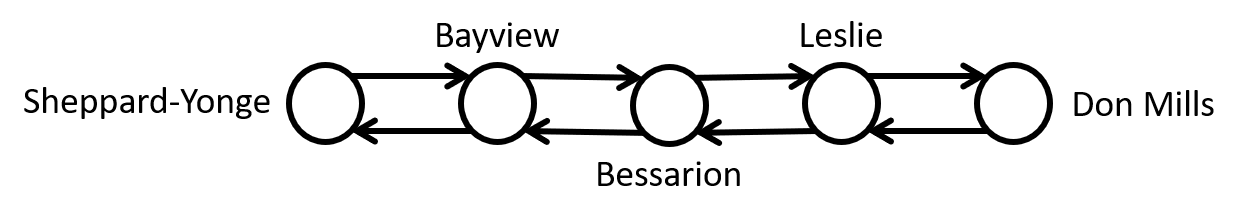
\includegraphics[width=6.5in]{directedgraph.png}
	\caption{Directed Graph Model of Sheppard Subway Line}\label{fig:directedgraph}
\end{figure}

What the directed graph representation lacks for this application is any notion
of an integrated train model. A separate train model could be made to use the
directed graph simply to know where to go next, but it would require much extra
logic to determine \textit{if} it could go do the next station.  Where this
decision is made is also not obvious when using the directed graph.

Similar to directed graphs and used in discrete event modeling of concurrent
systems is a structure called a Petri net.~\cite{Petri62}  Synonymous to the
vertices in a directed graph, Petri nets contain \textit{places}.  Whereas
directed graphs use edges to connect those vertices, Petri nets use
\textit{arcs}. However, Petri nets do not simply connect one \textit{place} to
another.  \textit{Arcs} actually connect \textit{places} to
\textit{transitions}. Each \textit{transition} has an input and an output arc
joining it to \textit{places}.  Each \textit{place} optionally can contain a
finite number of \textit{tokens}.  \textit{Tokens} for this application
represent the trains.  More formally, they are objects that represent processes
in a given state, where the states are represented by the
\textit{places}.~\cite{Kristoffersen2003}  Figure~\ref{fig:petrinet} shows a
Petri net model of the Sheppard subway line. The rectangles at the midpoint of
the arcs represent the transitions and the black dots inside the represent the
tokens.
%
\begin{figure}[htb]
	\centering
	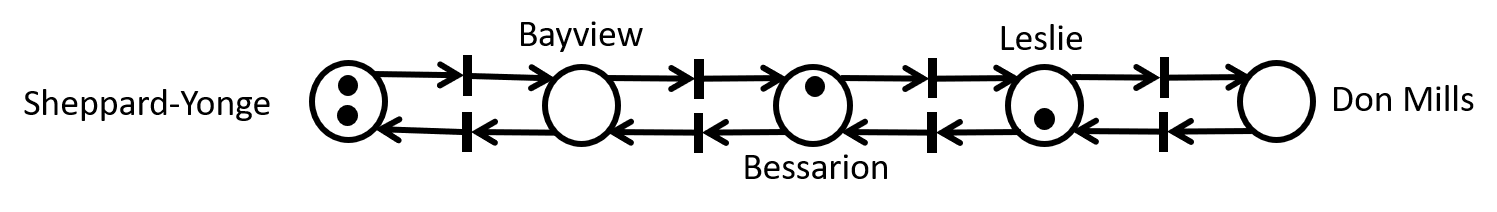
\includegraphics[width=6.5in]{petrinet.png}
	\caption{Petri Net Model of Sheppard Subway Line}\label{fig:petrinet}
\end{figure}
%

Collision detection and avoidance offers another method for simulating subways.
Collision detection is a method for simulating potentially colliding objects
moving in a space as a difference equation. Collisions are determined by
figuring out where all the objects would be in the next time instance if there
were not any collisions and figuring out which objects cross paths. Objects that
cross paths have collided and need to have their positions in the next time
period adjusted. In subway systems, collision detection with a directed graph model of the subway system can ensure feasible, crash free subway dynamics by requiring trains to be far enough apart that if one train stops the trains behind it does not rear end it. Calculation of minimum safe distance between trains requires information
about track layout and train velocity and acceleration. 

A model of a train traveling between stations has been done by Xu~\cite{Xu2014}. In their model of a train traveling between stations there is an acceleration period, a cruising period and a deceleration period. At each time step trains proceed to the next station in a safe manner taking into account time and energy efficiency. The safety criterion requires that the minimum stopping distance of the rear train is less than the distance between the leader and follower train train plus the minimum stopping distance of the lead train and a safety factor. 

Petri nets were chosen over collision detection for simulating subway train
movement because Petri nets are simpler, more efficient, require less data to
calibrate and capture the dynamics of train break downs and delays. Petri nets are simpler than collision detection because Petri nets do not have
the detailed physics requirements of a collision detection model. In the
collision detection model minimum safe distance needs to be calculated by every
train at every time step. With a Petri net, minimum safe distance calculations
can be avoided by discretizing the track into sections with length greater than
the trains minimum stopping distance at maximum speed (or with a number of
sections if a more than one track lookahead rule is used) which ensures that
collisions are always avoidable. Petri nets are more efficient because they do not require any physics calculations during simulation and can evaluated as discrete events which results in a fewer number of calculations being required so long as track sections are large relative to the size of the time steps in a collision model. Petri nets are capable of modeling the breakdown and delay dynamics of interest because a train delay or breakdown will back up the trains behind it so long as the section of track the delayed or broken down train is on does not have a
passing track. More data is needed for a collision detection model because it has higher physics fidelity than a Petri net. With the Petri net you only need the time it takes to pass through a section of track and the minimum stopping distance at
maximum speed. The collision model requires knowledge of train accelaration and
deceleration and maximum speed at different locations on the track.
